\documentclass[11en, a4paper, oneside]{article}
\usepackage[utf8]{inputenc}
\usepackage{graphicx}
\usepackage{amsmath}
\usepackage[bottom=3.0cm,top=3.0cm,left=3.0cm,right=3.0cm]{geometry}
\usepackage[portuguese]{babel}
\usepackage{indentfirst}
\usepackage{fancyhdr}
\usepackage{hyperref}
\usepackage{subfiles}
\usepackage{wrapfig}
\usepackage{subcaption}
\usepackage[utf8]{inputenc}
%\usepackage[nottoc]{tocbibind}
\usepackage{lastpage}
\newcommand{\clap}{\makebox[0pt]}
\usepackage{titlesec}
\usepackage{amsfonts}
\usepackage{listings}
\usepackage{color} %red, green, blue, yellow, cyan, magenta, black, white
\definecolor{mygreen}{RGB}{28,172,0} % color values Red, Green, Blue
\definecolor{mylilas}{RGB}{170,55,241}
\newcommand{\overbar}[1]{\mkern 1.5mu\overline{\mkern-1.5mu#1\mkern-1.5mu}\mkern 1.5mu}
\titleformat{\paragraph}
{\normalfont\normalsize\bfseries}{\theparagraph}{1em}{}
\titlespacing*{\paragraph}
{0pt}{3.25ex plus 1ex minus .2ex}{1.5ex plus .2ex}


\usepackage{etoolbox}
\patchcmd{\thebibliography}{\section*{\refname}}{}{}{}

\graphicspath{ {./Imagens/} }

\hypersetup{colorlinks,citecolor=black,filecolor=black,linkcolor=black,urlcolor=black} 

\lstset{language=Matlab,%
    %basicstyle=\color{red},
    breaklines=true,%
    morekeywords={matlab2tikz},
    keywordstyle=\color{blue},%
    morekeywords=[2]{1}, keywordstyle=[2]{\color{black}},
    identifierstyle=\color{black},%
    stringstyle=\color{mylilas},
    commentstyle=\color{mygreen},%
    showstringspaces=false,%without this there will be a symbol in the places where there is a space
    numbers=left,%
    numberstyle={\tiny \color{black}},% size of the numbers
    numbersep=9pt, % this defines how far the numbers are from the text
    emph=[1]{for,end,break},emphstyle=[1]\color{red}, %some words to emphasise
    %emph=[2]{word1,word2}, emphstyle=[2]{style},    
}


\pagestyle{fancy}
\fancyhf{}
\rhead{Circuit Theory and Electronics Fundamentals}
\lhead{Group 21}
\cfoot{Página  \thepage \hspace{1pt} de \pageref{LastPage}}
\pagenumbering{roman}

\begin{document}


\begin{titlepage}
	\begin{center}
		\begin{figure}[htb!]
			\begin{center}
				
\includegraphics[width=10cm]{tecnico.png}
			\end{center}
		\end{figure}
		
        \vspace{30pt}
        \begin{center}
        \Large{\center Integrated Masters in Aerospace Engineering, Técnico, University of Lisbon}\\
        \Large{\center Circuit Theory and Electronics Fundamentals}\\
        \end{center}
            
        \vspace{60pt}
        \Huge{\textbf{Laboratory Report 1}}
        
        \vspace{120pt}
        \begin{minipage}{0.4\textwidth}
		\begin{flushleft} \large
			\emph{\LARGE{\textbf{Grupo 21:}}}\par \vspace{10pt}
			95791, Francisco Carvalho \\ \vspace{20pt}
            95805, João Matias\\ \vspace{20pt}
            95846, Simão Gonçalves\\ \vspace{20pt}
		\end{flushleft}
	\end{minipage}
	~
	\begin{minipage}[b]{0.4\textwidth}
		\begin{flushright} \large
        	{}
		\end{flushright}
	\end{minipage}\\[2cm]
       \vspace{10pt}
        \large{March 25th 2021}\\
	\end{center}
\end{titlepage}

\newpage
\renewcommand{\contentsname}{Índice}
\tableofcontents
\thispagestyle{empty}

\newpage
\pagenumbering{arabic}
\setcounter{page}{3}

\section{Introduction}

For the first experimental activity in the Circuit Theory and Electronics Fundamentals course, we were given a simple circuit to analyse, in relation to the contents presented in the first three weeks of the semester.
This circuit is constituted by a dependent and independent voltage source, a dependent and independent current source and 7 resistors (fig. \ref{intro}).
In order to solve the circuit we performed a theoretical analysis, using the node and mesh methods (Section \ref{sec:analysis}), and a simulation, using the software NGSpice (Section \ref{simuanal}). We then compared both results and tried to validate our theoretical analysis (Section \ref{resan}).

\begin{figure}[htb!]
			\begin{center}
				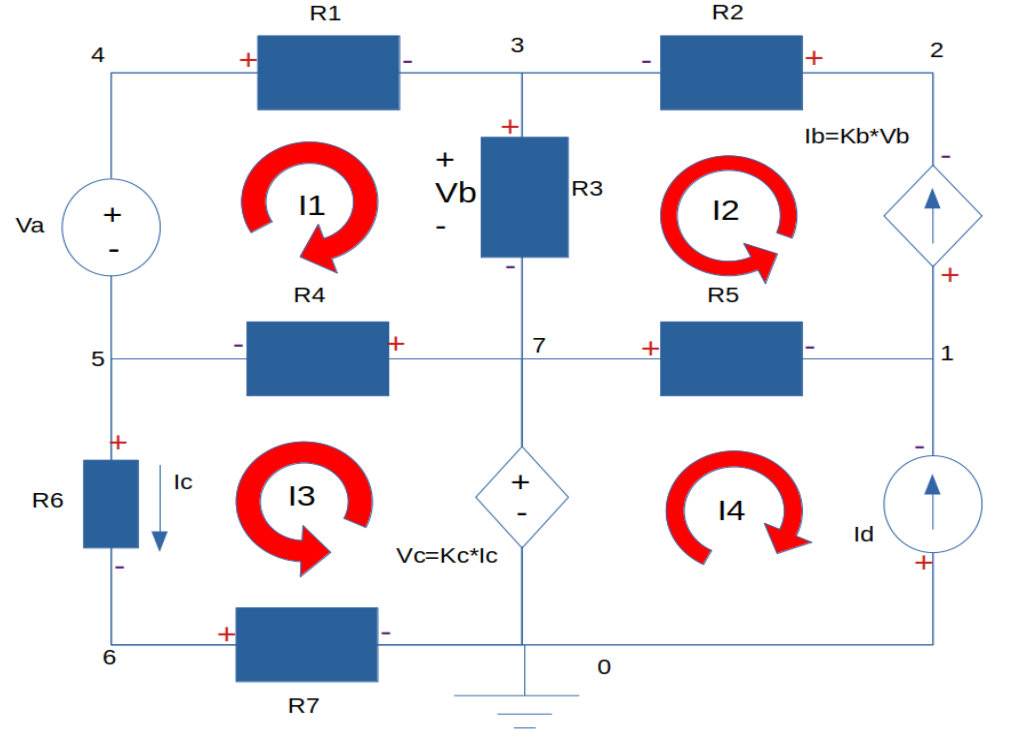
\includegraphics[width=10cm]{Intro.png}
				\caption{Analyzed Circuit}
				\label{intro}
			\end{center}
\end{figure}

To obtain the initial data, we ran a python script provided by our teacher, which generated the following data:\\

\begin{table}[ht]
\begin{center}
\begin{tabular}{|l|l|}
\hline
\textbf{Name} & \textbf{Generated Data} \\ \hline
R1        & 1.04899828982           \\ \hline
R2        & 2.0555682231            \\ \hline
R3        & 3.06018802573           \\ \hline
R4        & 4.16897961659           \\ \hline
R5        & 3.07395007732           \\ \hline
R6        & 2.0428100493            \\ \hline
R7        & 1.03756256625           \\ \hline
Va        & 5.11422921556           \\ \hline
Id        & 1.01155034907           \\ \hline
Kb        & 7.33855517177           \\ \hline
Kc        & 8.2581000183            \\ \hline
\end{tabular}
\caption{Inicial data. Resistors and Kc in kOhm, Voltage in V, Current inmA and Kb in mS}
\end{center}
\end{table}

\clearpage

\section{Theoretical Analysis}
\label{sec:analysis}

In this section, we expose and explain the methods used to solve and analyse the circuit. In this specific case: the Mesh and the Node Methods.

\subsection{Mesh Method}

The Mesh Analyses consists in defining circulating currents in all the simple meshes, and then calculating them. So, 
with this method we determine the currents I1, I2, I3 and I4. This results were achieved looking to the  loop formed by R1, R3, R4 and Va and other loop formed by R4, R6, R7 and Vc. The circulating currents are I1 and I3, respectively.  The third independent equation were obtained equaling I2 to Kb*Vb and Vb to (I2+I3)*R3. The last and fourth equation is a very simple one, we just equal I4 to -Id. To solve this system of linear equations we  rearranged them in the matrix form below, and we obtained the solution using Octave math tools.\\

$\begin{bmatrix}
R1+R3+R4 & -R3 & -R4 & 0\\
   
-R4 & 0 & -Kc+R4+R6+R7 & 0\\

-Kb*R3 & Kb*R3-1 & 0 & 0\\

0 & 0 & 0 & 1
\end{bmatrix}$
$\begin{bmatrix}
I1\\
I2\\
I3\\
I4
\end{bmatrix}$
= 
$\begin{bmatrix}
Va\\
0\\
0\\
-Id
\end{bmatrix}$

\begin{table}[ht]
\begin{center}
    \begin{tabular}{|l|l|}
\hline
\textbf{Name} & \textbf{Value {[}A{]}} \\ \hline
I1            & 0.00022930             \\ \hline
I2            & -0.00023999            \\ \hline
I3            & 0.00094758             \\ \hline
I4            & -0.00101155            \\ \hline
\end{tabular}
\caption{Circulating currents obtained through the application of the Mesh Method in Octave}
\end{center}
\end{table}

\begin{table}[h]
\begin{center}
\begin{tabular}{|l|l|}
\hline
\textbf{} & \textbf{Resistor's Current} \\ \hline
R1(i)     & 2.2930e-4                   \\ \hline
R2(i)     & -2.3999e-4                  \\ \hline
R3(i)     & -1.069e-5                   \\ \hline
R4(i)     & 1.17688e-3                  \\ \hline
R5(i)     & -1.25154e-3                 \\ \hline
R6(i)     & 9.4758e-4                   \\ \hline
R7(i)     & 9.4758e-4                   \\ \hline
\end{tabular}
\caption{Current values through each Resistor}
\end{center}
\end{table}

\subsection{Node Method}
The objective of this method is to determine every node voltage. To do this we have to first number nodes arbitrarily, assign potential 0V (Ground) to one of the nodes, and then calculate all the voltages. We had 7 unknown variables, so we determined 7 independent equations. This equations were obtained doing KCL in nodes 1,2,3,6 and 7; knowing that Va=V4-V5; and using the fact that V7 equals Vc, that in turn equals Kc*Ic. The equations were rearranged in the matrix form below, in order to find the solution using Octave math tools.\\


$\begin{bmatrix}
G5 & 0 & Kb & 0 & 0 & 0 & -Kb-G5\\
0 & G2 & Kb-G2 & 0 &  & 0 & Kb\\
0 & -G2 & G1+G2+G3 & -G1 & 0 & 0 & -G3\\
0 & 0 & 0 & 0 & -G6 & G7+G6 & 0\\
-G5 & 0 & -G3 & 0 & -G4 & -G7 & G3+G4+G5\\
0 & 0 & 0 & 1 & -1 & 0 & 0\\
0 & 0 & 0 & 0 & 0 & Kc*G7 & -1
\end{bmatrix}$
$\begin{bmatrix}
V1 \\ V2 \\ V3 \\ V4 \\ V5 \\ V6 \\ V7
\end{bmatrix}$
= 
$\begin{bmatrix}
Id \\ 0 \\ 0 \\ 0 \\ -Id \\ Va \\ 0
\end{bmatrix}$
 
\paragraph{}
\begin{table}[ht]
\begin{center}
\begin{tabular}{|l|l|}
\hline
\textbf{Name} & \textbf{Value {[}V{]}} \\ \hline
V1            & 11.67246               \\ \hline
V2            & 7.29929                \\ \hline
V3            & 7.79260                \\ \hline
V4            & 8.03313                \\ \hline
V5            & 2.91891                \\ \hline
V6            & 0.98318                \\ \hline
V7            & 7.82530                \\ \hline
\end{tabular}
\caption{Node's voltage obtained through the application of the Node Method in Octave}
\end{center}
\end{table}

\par With these results, we are able to compare both methods. Calculating $(V4-V3)/R1$ with the voltages of the node method we get I1. Repeating the same process for V2, V3 and R2 we obtain I2 and for V5, V6 and R6 we get I3. The calculations lead us to the following table:

\begin{table}[ht]
\begin{center}
    \begin{tabular}{|l|l|}
\hline
\textbf{Name} & \textbf{Value {[}A{]}} \\ \hline
I1            & 0.00022930             \\ \hline
I2            & -0.00023999            \\ \hline
I3            & 0.00094758             \\ \hline
I4            & -0.00101155            \\ \hline
\end{tabular}
\caption{Current results}
\end{center}
\end{table}

Just like we expected, the results of both methods are coincident. Therefore, we can conclude that the two analyses are correct.

\newpage
\section{Simulation Analysis}
\label{simuanal}
With the objective of solving the given circuit, we began by drawing a sketch of it, which can be seen in the picture below.

\begin{figure}[htb!]
			\begin{center}
				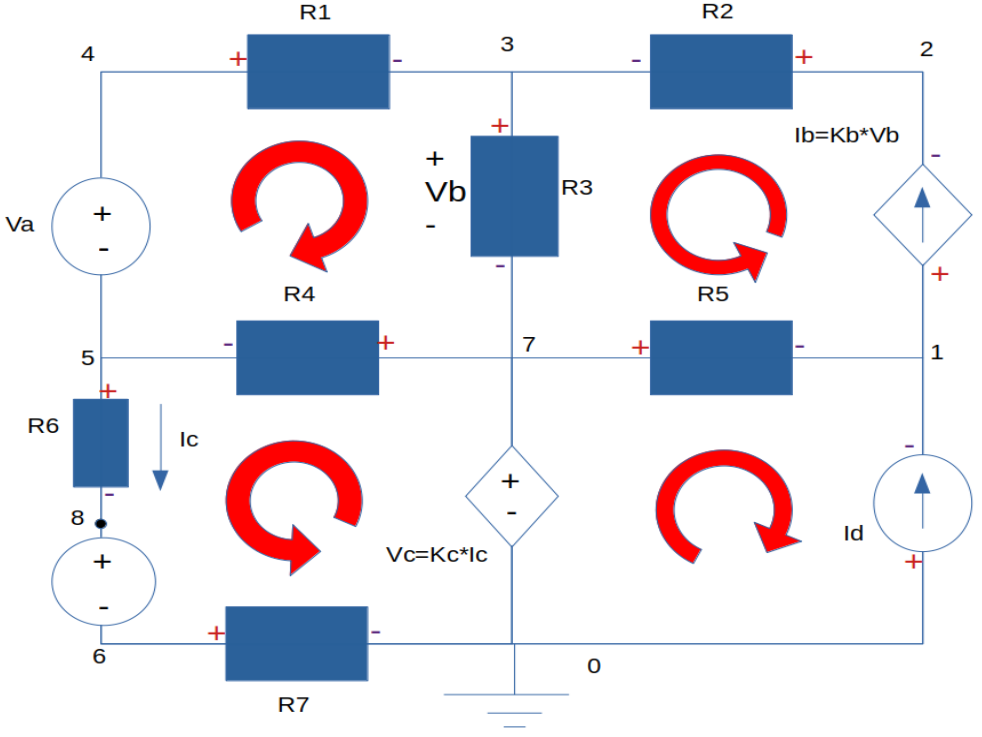
\includegraphics[width=10cm]{Simulacao.png}
				\caption{Analyzed Circuit in NGSpice}
			\end{center}
\end{figure}

In order to understand our approach, it is important to note the following:

- We considered the node to which we connect resistor R7, Current Source Id and Dependent Voltage Source Vc to be the ground (node 0 in the picture).

-To compute the voltage drop through the dependent voltage source (Vc), we needed to obtain the current value through resistor R6. However, NGSpice doesn't allow us to input Resistor R6 current in the computation. Hence, in order to solve this problem, we consulted an online forum which stated that this problem could be solved by introducing a voltage source with no voltage drop in series with the R6 resistor. This way, we managed to obtain the current through it, and therefore we were able to compute the dependent voltage source Vc.

NGSpice is a really useful tool, which allows us to compute the circuit and obtain all the necessary parameters. After carefully writing the script, in which we specify the nodes where we connect every single component and create the necessary dependencies for the dependent sources, we obtain the following table after typing the \textit{ngspice script.name} command in a terminal window.

In this table, we can see the voltage at any given node, the current through each resistor and the voltage and current sources. (We use the ngspice terminology: @-current value; Also, voltage value at node 0 (0V) is not shown)
\clearpage
\begin{table}[h]
\label{tab1}
\begin{center}
\begin{tabular}{|l|r|}
\hline
\textbf{Name}    & \textbf{Value (A or V)} \\\hline
@gb{[}i{]}       & -2.39986e-04            \\\hline
@id{[}current{]} & 1.011550e-03            \\\hline
@r1{[}i{]}       & 2.293000e-04            \\\hline
@r2{[}i{]}       & -2.39986e-04            \\\hline
@r3{[}i{]}       & -1.0686e-05             \\\hline
@r4{[}i{]}       & 1.176882e-03            \\\hline
@r5{[}i{]}       & -1.25154e-03            \\\hline
@r6{[}i{]}       & 9.475818e00             \\\hline
@r7{[}i{]}       & 9.475818e00             \\\hline
v(1)             & 1.167246e+01            \\\hline
v(2)             & 7.299291e+00            \\\hline
v(3)             & 7.792599e+00            \\\hline
v(4)             & 8.033134e+00            \\\hline
v(5)             & 2.918905e+00            \\\hline
v(6)             & 9.831754e-01            \\\hline
v(7)             & 7.825301e+00            \\\hline
v(8)             & 9.831754e-01         \\\hline

\end{tabular}
\caption{Results from NGSpice} \label{tab:sometab}
\end{center}
\
\end{table}



\section{Results Analysis, Errors and Conclusion}
\label{resan}
After performing the computation, it's time to compare its' results to the ones obtained theoretically, through the application of the mesh and node methods with the help of Octave's math tool. In order to do so, we will calculate the error for every single value obtained.

\begin{table}[h]
\begin{center}
\begin{tabular}{|l|l|}
\hline
\textbf{Name}    & \textbf{Relative Error (\%)} \\\hline
V1 & 0           \\\hline
V2 & 1.37000e-05 \\\hline
V3 & 1.28327e-05 \\\hline
V4 & 4.97938e-05 \\\hline
V5 & 1.71297e-04 \\\hline
V6 & 4.67870e-04 \\\hline
V7 & 1.27791e-05 \\\hline
IA & 1.30833e-04 \\\hline
IB & 1.58757e-03 \\\hline
IC & 1.87847e-04 \\\hline
\end{tabular}
\caption{Relative Error between Octave's and NGSpice's values}
\end{center}
\end{table}

As we can see the error values are minimal for every single component of the circuit. Even though we could have expected a bigger error margin due to the number of circuit components, that was not the case. The main reason for this perfect match between computation results and theoretical results is the circuit simplicity, since its components are only DC voltage sources, current sources and resistors. We believe that the main cause for errors was probably because of rounding issues, due to Octave's limited floating point representation.
\end{document}

